\input{../../../headers/dsheaders.tex}

\section*{Introduction}

Pharmathek, entreprise basée à Vérone en Italie et implantée en France dans la région de Nancy, a mis au point un robot de stockage, de rangement et de délivrance des ordonnances, permettant aux pharmacies équipées de s'affranchir de la pénibilité de la gestion manuelle des boîtes de médicaments.

Les missions du robot SINTESI sont de diminuer le nombre d'aller-retours effectués par les collaborateurs en pharmacie entre le comptoir et les tiroirs de stockage des médicaments, de faciliter le stockage des références qui arrivent chaque jour et d'augmenter le temps de présence et de conseil aux patients.

\textbf{Remarque :} afin de respecter la confidentialité de ce système, les données et résultats présentés dans ce sujet sont approchés et limitatifs par rapport à la solution industrielle réelle.

\begin{figure}[ht!]
\centering

\includegraphics[width=0.7\textwidth]{img/fig01}
\caption{\label{fig01}Robot SINTESI avec un seul bras et sa tête SLIM ou sa tête EUCLID3D}
\end{figure}

Le robot SINTESI se présente sous la forme d'un couloir d'environ 60 cm de large, bordé à gauche et à droite par deux magasins de stockage. Chaque magasin possède des étagères en verre de différentes hauteurs avec une profondeur utile de stockage d'environ 35 cm. Le robot comporte ensuite un ou deux bras manipulateurs trois axes (ici un seul bras situé sur la droite de la photo), munis d'une tête de manipulation des boîtes dont deux versions sont proposées : la tête SLIM ou la tête EUCLID3D.

Le chargement des boîtes de médicaments dans le robot est hors du cadre de cette étude.

Ce sujet a pour but d'élaborer un modèle de simulation devant permettre d'apporter une aide décisionnelle sur le choix de la tête à implanter. Les résultats de simulation devront faire apparaître les écarts de performances du robot muni d'une tête simple (nommée SLIM) vis-à-vis d'une tête plus perfectionnée (nommée EUCLID3D).

Le robot SINTESI doit répondre aux exigences de la figure \ref{fig02} qui seront validées tout au long du sujet.

\begin{figure}[ht!]
\centering

\includegraphics[width=\textwidth]{img/fig02}
\centering
\begin{tabular}{|m{2cm}|m{5.5cm}|m{8cm}|}
\hline
\textbf{Exigence} & \textbf{Performance} & \textbf{Niveau} \\
\hline
\multirow{8}{2cm}{Pilotage des axes} & \multirow{2}{3cm}{Précisions des axes X et Z} & Erreur en régime permanent pour une consigne en échelon inférieure à 0,5 mm \\ \cline{3-3}
 & & Erreur de traînage en régime permanent pour une consigne en rampe (vitesse maximale) inférieure à 50 mm \\ \cline{2-3}
 & \multirow{2}{5.5cm}{Stabilité des asservissements de position} & Marge de phase minimale de 45° \\
 \cline{3-3}
 & & Dépassement de l'axe Thêta inférieur à 1°\\
 \cline{2-3}
 & Vitesses des axes X et Z & Vitesse maximale $v_{\max} = 2{,}5~\text{m} \cdot \text{s}^{-1}$ \\
 \cline{2-3}
 & Vitesse de l'axe Thêta & Vitesse maximale de $100^\circ \cdot \text{s}^{-1}$ \\
 \cline{2-3}
 & Accélérations des axes X et Z & Accélération maximale de $a_{\max} = 2~\text{m} \cdot \text{s}^{-2}$ \\ \cline{2-3}
 & Accélération de l'axe Thêta & Accélération maximale de $400^\circ \cdot \text{s}^{-2}$ \\
\hline
\end{tabular}
\caption{\label{fig02}Diagramme et tableau des exigences partielles du robot SINTESI}
\end{figure}

Certaines questions, peu ou pas guidées, demandent de l'initiative de la part du candidat. Il est alors demandé d'expliciter clairement la démarche, les choix et de les illustrer, le cas échéant, par un schéma. Le barème valorise la prise d'initiative et tient compte du temps nécessaire à la résolution de ces questions.

\section{Modélisation du robot SINTESI}

\paragraph{Objectif} Analyser la structure du robot et établir des modèles comportementaux.

\subsection{Architecture du bras manipulateur 3 axes}

\paragraph{Objectif} Analyser la cinématique du bras manipulateur.

Le bras manipulateur comprend trois axes : l'axe X, l'axe Z et l'axe Thêta dont la figure \ref{fig03} et le tableau \ref{tab01} précisent l'architecture.

\begin{figure}[ht!]
\centering

\includegraphics[width=0.76\textwidth]{img/fig03}
\caption{\label{fig03}Architecture du manipulateur 3 axes}
\end{figure}

\newpage

\begin{table}[ht!]
\centering
\begin{tabular}{|p{4.5cm}|p{3.5cm}|p{3.5cm}|p{3.5cm}|}
\hline
\textbf{Axe} & \textbf{Axe X} & \textbf{Axe Z} & \textbf{Axe Thêta} \\
\hline
Courses & de 0 à 10 m & de 0 à 2,5 m & de $\theta_{\min}$ à $\theta_{\max}$ \\
\hline
Pièces considérées & 10 par rapport à 0 & 20 par rapport à 10 & 30 par rapport à 20 \\
\hline
Mouvements & Translation de direction $\vec{X}$ & Translation de direction $\vec{Z}$ & Rotation autour de l'axe $(F,\vec{Z})$ \\
\hline
Paramètres de position & $x(t)$ & $z(t)$ & $\theta(t)$ \\
\hline
\end{tabular}
\caption{\label{tab01}Paramétrage des mouvements des trois axes du robot}
\end{table}

Le schéma cinématique à compléter est fourni sur le document réponse.

\question{À l'aide du tableau \ref{tab01}, proposer un graphe des liaisons d'une modélisation minimale restreinte aux solides \textbf{0}, \textbf{10}, \textbf{20}, \textbf{30}.}

\question{Compléter l'épure du document réponse en représentant les liaisons correspondant au graphe des liaisons précédent.}

~\

Le diagramme de définition de blocs du robot, dans la configuration étudiée (avec tête EUCLID3D), est donné à la figure \ref{fig04}.

\begin{figure}[ht!]
\centering

\includegraphics[width=\textwidth]{img/fig04}
\caption{\label{fig04}Diagramme de définition de blocs du robot SINTESI}
\end{figure}

Le paramétrage est fourni dans le tableau \ref{tab02}.

\question{À l'aide du paramétrage et des valeurs figurant dans le tableau \ref{tab02} et sur le document réponse de la question \ref{q2}, déterminer les expressions littérales et les valeurs numériques des paramètres $\rho_1$ et $\rho_x$ tels que $\omega_{12}(t) = \rho_1 \omega_{11}(t)$ et $v_x(t) = \rho_x \omega_{11}(t)$ en précisant l'unité de $\rho_x$.}

\newpage

\begin{table}[ht!]
\begin{tabular}{|m{0.5cm}|m{2cm}|m{3cm}|m{3.5cm}|m{6cm}|}
\hline
\textbf{Sol.} & \textbf{Nom} & \textbf{Repère associé} & \textbf{Paramétrage des mouvements} & \textbf{Masse et grandeurs cinétiques} \\
\hline
0 & Bâti & $(O,\vec{X},\vec{Y},\vec{Z})$ & & \\
\hline
10 & Chariot & $(A,\vec{X},\vec{Y},\vec{Z})$ & $\overrightarrow{OA} = x(t)\vec{X}$ 

$\vec{V}_{10/0}(A) = v_x(t)\vec{X}$

$\vec{a}_{10/0}(A) = a_x(t)\vec{X}$

$v_x(t) = \rho_x \omega_{11}(t)$ & $m_{10} = 20$ kg \\
\hline
11 & Rotor moteur axe X & $(B,\vec{X}_{11},\vec{Y}_{11},\vec{Z})$ & $\vec{\Omega}_{11/10} = \omega_{11}(t)\vec{Z}$

$v_x(t) = \rho_x \omega_{11}(t)$ & Masse $m_{11} = 5{,}3$ kg et moment d'inertie $I_{11} = 7,5 \cdot 10^{-5}$ kg$\cdot$m$^2$ par rapport à l'axe $(B,\vec{Z})$ et équilibré autour de cet axe. \\
\hline
12 & Arbre de transmission & $(C,\vec{X}_{12},\vec{Y}_{12},\vec{Z})$ & $\vec{\Omega}_{12/10} = \omega_{12}(t)\vec{Z}$

$\omega_{12}(t) = \rho_1 \omega_{11}(t)$ & Masse $m_{12} = 14$ kg et moment d'inertie $I_{12} = 1{,}6 \cdot 10^{-4}$ kg$\cdot$m$^2$ par rapport à l'axe $(C,\vec{Z})$ et équilibré autour de cet axe. \\
\hline
13 & Rotor moteur axe Z & $(E,\vec{X},\vec{Y}_{13},\vec{Z}_{13})$ & $\vec{\Omega}_{13/10}$ & Masse $m_{13} = 5{,}76$ kg \\
\hline
20 & Ascenseur & $(D,\vec{X},\vec{Y},\vec{Z})$ & $\overrightarrow{AD} = z(t)\vec{Z}$ & $m_{20} = 10$ kg \\
\hline
30 & Tête & $(F,\vec{X}_{30},\vec{Y}_{30},\vec{Z})$ & $\overrightarrow{FG_{30}} = R_{30}\vec{Y}_{30}$

$\vec{\Omega}_{30/20} = \omega(t)\vec{Z}$

$\theta_{30/20} = \theta(t)\vec{Z}$ & Masse $m_{30} = 15$ kg et moment d'inertie $I_{30} = 0{,}8$ kg$\cdot$m$^2$ par rapport à l'axe $(G_{30},\vec{Z})$. \\
\hline
31 & Rotor moteur axe Thêta & $(H,\vec{X}_{31},\vec{Y}_{31},\vec{Z})$ & $\vec{\Omega}_{31/20} = \omega_{31}(t)\vec{Z}$ & Masse et inertie négligées. \\
\hline
\multicolumn{5}{|l|}{\textbf{hypothèses supplémentaires :} la masse des courroies, les masses et les inerties}\\
\multicolumn{5}{|l|}{de toutes les poulies et de tous les galets sont négligées.} \\
\hline
\end{tabular}
\caption{\label{tab02}Paramétrage dimensionnel et cinétique}
\end{table}

\subsection{Analyse des déplacements mesurés}

\paragraph{Objectif} Analyser la stratégie de pilotage des axes du robot.

\begin{figure}[ht!]
\begin{minipage}{0.39\linewidth}
Une campagne de mesures, à l'aide d'un accéléromètre (nommé module AHRS - Attitude and Heading Reference System - sur la figure \ref{fig05}) placé sur la tête EUCLID3D, a été effectuée.
\end{minipage}\hfill
\begin{minipage}{0.59\linewidth}
\centering

\includegraphics[width=0.7\textwidth]{img/fig05}
\caption{\label{fig05}Implantation du module AHRS}
\end{minipage}
\end{figure}

~\

Le fichier de points récupéré est un fichier au format csv. Après traitement sous Python, les trois tableaux Numpy ci-dessous à une dimension sont créés :
\begin{itemize}
\item \texttt{temps} : vecteur des temps avec une période d'échantillonnage constante $T_e = 0{,}01$ s, $\texttt{temps}[i]$ est donc égal à $iT_e$ ;
\item \texttt{ax} : vecteur des accélérations selon $\vec{X}$, $\texttt{ax}[i]$ est donc la valeur de l'accélération selon $\vec{X}$ à l'instant $i\cdot T_e$ ;
\item \texttt{az} : vecteur des accélérations selon $\vec{Z}$ (l'accélération de la pesanteur $\vec{g}$, qui est également mesurée par l'accéléromètre, est supposée compensée et donc n'est pas à prendre en compte).
\end{itemize}

Le tracé des accélérations brutes permet d'obtenir le graphe de la figure \ref{fig06}.

L'exploitation des mesures nécessite la mise en place d'un filtrage afin d'accéder aux accélérations moyennes du bras. Un filtre passe-bas, modélisé par une fonction du premier ordre, de gain unitaire et de constante de temps $\texttt{tau} = 5 \cdot T_e$ est appliqué aux vecteurs (en entrée) \texttt{ax} et \texttt{az} pour donner respectivement les vecteurs (en sortie) \texttt{axf} et \texttt{azf}.

\question{Donner l'équation différentielle temporelle qui lie les grandeurs $a_x(t)$ et $a_{xf}(t)$.}

~\

Soit le schéma de calcul suivant:  
$\dfrac{da_{xf}}{dt} \simeq \dfrac{\texttt{axf}[i] - \texttt{axf}[i-1]}{T_e}$

\question{Déterminer l'équation de récurrence sur les vecteurs \texttt{ax} et \texttt{az}. Le résultat sera présenté sous la forme $\texttt{axf}[i] = A \cdot \texttt{axf}[i-1] + B \cdot \texttt{ax}[i]$ où les constantes $A$ et $B$ seront exprimées en fonction de $T_e$ et de $\texttt{tau}$.}

\begin{figure}[ht!]
\centering

\includegraphics[width=0.45\textwidth]{img/fig06}
\caption{\label{fig06}Graphes des accélérations brutes sous Python}
\end{figure}

Le début du script permettant de définir le vecteur (liste) \texttt{axf} est donné ci-dessous. La liste
\texttt{ax} est considérée comme définie au préalable.

\begin{minted}[linenos]{python}
N=len(ax)
axf=[0]*N
axf[0]= ax[0]
Te = 0.01
tau = 5*Te
A=
\end{minted}

\question{Compléter le script précédent pour définir le vecteur \texttt{axf}, correspondant au résultat du filtre passe-bas du premier ordre sur le vecteur connu \texttt{ax}.}

\question{En sachant que $axf(t)=\dfrac{Vxf(t)}{dt}$ et en utilisant le schéma de calcul précédent, donner la suite du script python qui permet de calculer \texttt{vxf} à partir de \texttt{axf}.}

~\

À l'aide d'une nouvelle intégration, puis en appliquant aussi ces scripts selon $\vec{Z}$, les tracés de la figure \ref{fig07} sont obtenus.

\begin{figure}[ht!]
\centering

\includegraphics[width=0.7\textwidth]{img/fig07}
\caption{\label{fig07}Graphes des grandeurs cinématiques filtrées sous Python}
\end{figure}

\question{À l'aide de la figure \ref{fig07}, estimer les valeurs maximales des accélérations et des vitesses mesurées selon $\vec{X}$. Analyser les différences entre les résultats de mesures et les spécifications figurant dans le tableau des exigences figure \ref{fig02}.}

~\

Dans ce cas particulier, c'est l'axe X qui impose le temps de déplacement complet puisque l'amplitude du déplacement selon $\vec{X}$ est supérieure à celle selon $\vec{Z}$. Dans la suite du sujet, la vérification du dimensionnement de la motorisation se fera uniquement sur l'axe $X$.

\subsection{Modélisations de l'axe X}

\paragraph{Objectif}
Renseigner les paramètres de modèles comportementaux du bras en translation selon $\vec{X}$.

\begin{figure}[ht!]
\centering

\includegraphics[width=0.5\textwidth]{img/fig08}
\caption{\label{fig08}Profil simplifié des vitesses utilisé}
\end{figure}

Le profil de pilotage utilisé par le constructeur suit un profil en trapèze des vitesses. Dans le cas de l'amplitude de déplacement étudiée de 2,7 m, ce profil se simplifie en un triangle des vitesses symétrique (voir figure \ref{fig08}) puisque la vitesse maximale ne peut pas être obtenue pendant le déplacement limité de 2,7 m.

Les valeurs des accélérations utilisées sont les accélérations maximales spécifiées dans le tableau des exigences. On considère l'origine des temps au début du mouvement.

\question{Tracer les allures des évolutions temporelles de l'accélération $a_x(t)$ et du déplacement $x(t)$ en précisant les valeurs caractéristiques ($a_x(0)$, $a_x(t_1)$, $a_x(t_2)$, $v_x(0)$, $v_x(t_1)$, $v_x(t_2)$, $x(0)$, $x(t_1)$ et $x(t_2)$) en fonction de $t_1$, $t_2$ et $v_1$.}

\question{Après avoir déterminé $v_1$ en fonction de $a_{\max}$ et $t_1$, déterminer le temps de mouvement $t_2$ permettant d'effectuer 2,7 m selon $\vec{X}$ avec ce profil des vitesses.}

\subsection{Validation du dimensionnement de l'axe X}

\paragraph{Objectif} Valider le choix de la motorisation de l'axe X.

Dans la suite du sujet, un modèle causal simplifié ou un modèle acausal seront utilisés suivant les parties d'étude et les performances à valider. Ces deux types de modélisation, pour le moteur seul, sont rappelés à la figure \ref{fig12}, $J$ étant l'inertie du rotor du moteur. Le schéma électrique du moteur de la figure \ref{fig11} sera utile pour la suite.

Les caractéristiques de la machine sont données dans le tableau \ref{tab03}.

\begin{table}[ht!]
\centering
\begin{tabular}{|m{5.8cm}|m{2.5cm}|m{4cm}|m{2.5cm}|}
\hline
\multicolumn{4}{|c|}{\textbf{Moteur}} \\
\hline
\textbf{Grandeur} & \textbf{Valeur} & \textbf{Grandeur} & \textbf{Valeur} \\
\hline
Couplage des enroulements & étoile & Nombre de pôles & 6 \\
\hline
Tension nominale entre phases & 210 V & Constante de f.e.m & 0,5 V$\cdot$s$\cdot$rad$^{-1}$ \\
\hline
Couple rotor bloqué & 3,28 N$\cdot$m & Résistance phase & 8 $\Omega$ \\
\hline
Couple à vitesse nominale & 3,93 N$\cdot$m & Inductance phase & 19,3 mH \\
\hline
Puissance à vitesse nominale & 1235 W & Intensité de pointe & 9,49 A \\
\hline
Vitesse nominale & 3000 tr$\cdot$min$^{-1}$ & Intensité nominale & 4,2 A \\
\hline
Couple impulsionnel & 8,86 N$\cdot$m & & \\
\hline
\multicolumn{4}{|c|}{\textbf{Codeur incrémental}} \\
\hline
\multicolumn{2}{|l|}{2500 points par tour} & \multicolumn{2}{l|}{2 voies} \\
\hline
\end{tabular}
\caption{\label{tab03}Caractéristiques du moteur HDT B10S}
\end{table}

\begin{figure}[ht!]
\centering

\includegraphics[width=0.32\textwidth]{img/fig11}
\caption{\label{fig11}Modèle de la machine à courant continu équivalente}
\end{figure}

\begin{figure}[ht!]
\centering

\includegraphics[width=0.8\textwidth]{img/fig12}
\caption{\label{fig12}Modèles causal et modèle acausal de la MCC équivalente}
\end{figure}

Une simulation à vide ($C_r = 0$) du moteur de l'axe X a été réalisée. Les deux modèles ont été renseignés de façon à obtenir le même comportement dynamique que la machine réelle. La réponse à un échelon de tension de 320 V a donné les résultats de la figure \ref{fig13}.

\begin{figure}[ht!]
\centering

\includegraphics[width=0.8\textwidth]{img/fig13}
\caption{\label{fig13}Réponses à un échelon et zoom de l'évolution de vitesse}
\end{figure}

\question{Justifier l'ordre de grandeur de la valeur numérique du courant de démarrage du moteur.}

\question{À partir du modèle causal proposé à la figure \ref{fig12}, déterminer l'expression de $\dfrac{\Omega_m(p)}{U(p)}\Big|_{C_r=0}$ sous forme canonique.}

\question{À partir de la figure \ref{fig13}, retrouver la valeur de l'inertie $J$ qui a été renseignée dans les modèles et comparer cette valeur à celle du constructeur qui figure dans le tableau \ref{tab02}.}

Seul le mouvement de l'axe X est étudié dans cette partie. Ainsi, $\vec{\Omega}_{13/10} = \vec{0}$, $\vec{\Omega}_{30/20} = \vec{0}$ et $\vec{\Omega}_{31/20} = \vec{0}$.

Indépendamment des résultats précédents, les valeurs $J_{1eq} = 8 \times 10^{-3}$ kg$\cdot$m$^2$ et $\rho_x = 0,01$ m sont retenues pour la suite.

D'après le Théorème de l'Énergie Cinétique, on peut écrire :
$$C_m = \frac{J_{1eq}}{\rho_x} \cdot a_{\max}$$

Les pertes dans les transmissions sont supposées négligeables ainsi que les efforts résistants. La puissance intérieure à l'ensemble E se limite donc à la puissance délivrée par le moteur.

\question{Déterminer alors le couple $C_m$ nécessaire à fournir par le moteur de l'axe X pour l'accélération maximale du diagramme des exigences et comparer cette valeur à celle fournie dans le tableau \ref{tab03}.}

~\

Les paramètres du modèle de simulation de l'axe X sont maintenant connus. La même démarche peut être effectuée pour l'axe Z dont la motorisation est similaire à celle de l'axe X.

\section{Validation des performances du robot}

\paragraph{Objectif}
Valider les choix du constructeur par rapport aux performances attendues.

\subsection{Justification et dimensionnement des résistances de dissipation}

\paragraph{Objectif}
Vérifier la nécessité des résistances de dissipation et les dimensionner.

Le modèle acausal correspondant au déplacement aller et retour du robot selon $\vec{X}$ est présenté à la figure \ref{fig14}.

\begin{figure}[ht!]
\centering

\includegraphics[width=\textwidth]{img/fig14}
\caption{\label{fig14}Modèle de simulation de l'axe $X$}
\end{figure}

\newpage

Les résultats de simulation sont présentés à la figure \ref{fig15}.

\begin{figure}[ht!]
\centering

\includegraphics[width=0.8\textwidth]{img/fig15}
\caption{\label{fig15}Résultats de simulation pour un déplacement aller/retour selon $\vec{X}$ de 2,7 m}
\end{figure}

Ces résultats temporels ont été reproduits sur le document réponse avec une approximation de l'évolution temporelle du couple moteur, dont la valeur approchée sera estimée à $1.6N\cot m$.

\question{En assimilant le couple à sa valeur approchée, tracer sur le document réponse, l'allure de la puissance délivrée par le moteur.}

\question{Déterminer l'énergie (en $W\cdot h$) consommée et l'énergie (en $W\cdot h$) produite par le moteur pendant cette phase de fonctionnement.}

\subsection{Réglage des asservissements de position}

\subsubsection*{Objectif}
Régler les correcteurs des variateurs afin de valider les performances de positionnement.

Le robot pharmathek réalise des déplacements suivant les axes X et Z en fonction des consignes de position issues d'un logiciel spécifique de traitement d'ordonnances. En fonction des boites demandées, celui-ci recherche dans sa base l'emplacement des différentes boites et envoie aux variateurs les consignes de déplacement. Le bon fonctionnement du système dépend du réglage du correcteur de position en termes de stabilité et de suivi de consigne.

L'étude qui suit se limite au dimensionnement du correcteur de l'axe X. Bien que le traitement soit numérique, la période de traitement sera considérée très petite par rapport aux constantes de temps du système afin de traiter le problème avec les outils des systèmes linéaires continus et invariants.

\newpage

La structure globale de la boucle de position (documentation constructeur) est donnée à la figure \ref{fig16}.

\begin{figure}[ht!]
\centering

\includegraphics[width=.8\linewidth]{img/fig16}
\caption{\label{fig16} Structure de la boucle de position du variateur donnée par le constructeur}
\end{figure}

\question{Identifier les différentes boucles présentes dans la structure de la figure \ref{fig16}.}

~\

Les variateurs ont la possibilité d'être pilotés par un logiciel dédié. Deux essais, limités à la boucle de vitesse, avec des consignes en échelon de 300 et $1200$~tr$\cdot$min$^{-1}$ ont été réalisés afin d'établir un modèle simplifié de l'asservissement de vitesse. Les résultats des essais sont donnés à la figure \ref{fig17}.

% Figure 17 - Résultats des essais
\begin{figure}[ht!]
\centering

\includegraphics[width=.9\linewidth]{img/fig17}
\caption{\label{fig17} Résultats des essais à un échelon de vitesse}
\end{figure}

\question{Justifier le fait que les deux relevés ne présentent pas la même allure. Préciser le nom de l'élément du schéma bloc de la figure \ref{fig16} qui intervient.}

\question{Identifier les paramètres $K$ et $\tau$ du modèle du premier ordre de la boucle de vitesse tels que:
\[H(p) = \frac{\Omega_m(p)}{\Omega_c(p)} = \frac{K}{1+\tau p}\]}

\newpage

Pour l'étude du correcteur de position, l'asservissement de position non perturbé peut se modéliser par le schéma bloc donné à la figure \ref{fig18} dans lequel la boucle de vitesse est remplacée par sa fonction de transfert $H(p)$.

% Figure 18 - Schéma bloc de la boucle de position
\begin{figure}[ht!]
\centering

\includegraphics[width=.9\linewidth]{img/fig18}
\caption{\label{fig18} Schéma bloc de la boucle de position ($\omega_m(t) = \omega_{11}(t)$)}
\label{fig:schema_bloc_pos}
\end{figure}

Le codeur, de type incrémental (voir tableau \ref{tab02}), placé sur l'arbre moteur, délivre 2~500 points par tour sur 2 voies soit 10~000 points par tour.

\question{Déterminer la valeur de $K_{cod}$ en points$\cdot$rad$^{-1}$ puis celle de l'adaptateur de consigne $A$ en points$\cdot$m$^{-1}$.}

\question{Déterminer la résolution (en $rad$) du codeur incrémental et vérifier qu'elle est compatible avec les exigences de précision du tableau des exigences (figure \ref{fig02}).}

Le correcteur $C(p)$ est un correcteur proportionnel de valeur $K_p$. La fonction de transfert $H(p)$ sera prise égale à $H(p) = \frac{1}{1+\tau\cdot p}$ avec $\tau = 20$ms.

\question{Déterminer l'expression littérale de la fonction de transfert en boucle ouverte $FTBO(p)$.}

~\

Le diagramme de Bode de la fonction de transfert en boucle ouverte $FTBO(j\omega)$ lorsque $K_p = 1$ est donné sur le document réponse.

\question{A partir du diagramme de Bode, identifier les paramètres de la fonction de transfert $FTBO(j\omega)$. Conclure quant aux résultats obtenus précédemment.}

~\

Les variateurs des axes X et Z reçoivent les consignes de déplacement du logiciel de traitement des ordonnances. La loi d'évolution de la consigne est alors élaborée par le variateur en fonction du profil de vitesse défini figure \ref{fig08}.

\newpage

Le but du questionnement à venir est de vérifier si le système est capable de suivre une consigne de position de type « rampe », lorsque la vitesse est constante. Le schéma bloc de la figure \ref{fig18} peut se réduire à celui de la figure \ref{fig19} avec $K_1 = 70$ après réglage de $K_p$.

% Figure 19 - Schéma bloc équivalent
\begin{figure}[ht!]
\centering

\includegraphics[width=.8\linewidth]{img/fig19}
\caption{\label{fig19} Schéma bloc équivalent}
\label{fig:schema_equiv_pos}
\end{figure}

\question{Déterminer la fonction de transfert en boucle fermée, $FBF(p)=\dfrac{X(p)}{X_c(p)}$.}

\question{Déterminer l'erreur en régime permanent (erreur de traînage) $\Delta x_v = \lim\limits_{t\to\infty}\mu(t)$ en fonction de $K_1$ lorsque l'entrée de consigne de position est une rampe de pente $V_x$ constante. Il est rappelé la transformée de Laplace :
\[x_c(t) = V_x t \xrightarrow{\mathcal{L}} X_c(p) = \frac{V_x}{p^2}\]}

\vspace{-0.5cm}
\question{Conclure sur la capacité du système à suivre les lois d'évolution des consignes de position en translation vis-à-vis des exigences du tableau de la figure \ref{fig02}.}

%\finsujet{public}
\finsujet

\sautpage{2}
\debutcor

\reponse{4}{}{

\centering
   \def\svgwidth{0.5\textwidth}
   \input{img/cor01.pdf_tex}
}

\reponse{0}{

\centering

\includegraphics[width=0.7\textwidth]{img/dr02}}{

\centering
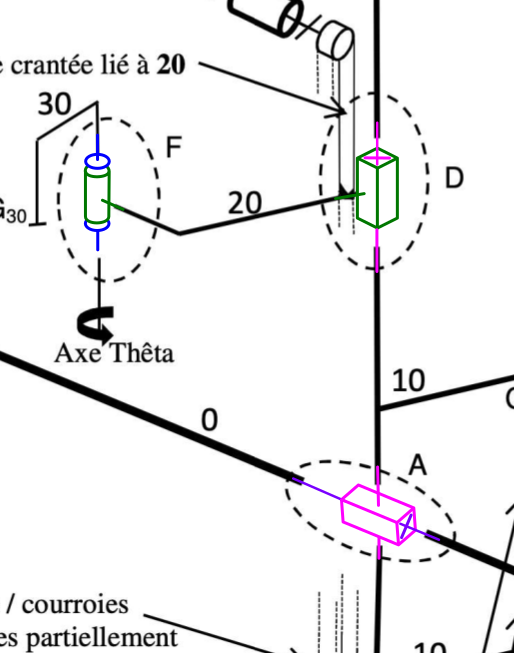
\includegraphics[width=0.4\textwidth]{img/cor02}
}

\reponse{5}{}{

$\rho_1 = \dfrac{\omega_{12}}{\omega_{11}} = \dfrac{R_{11}}{R_{12a}}$.

De plus, $v_x = R_{12b}\omega_{12}$ et $\omega_{12} = \rho_1 \omega_{11} \Longrightarrow v_x = R_{12b}\rho_1\omega_{11} = \rho_x\omega_{11}$.

Donc $\rho_x = R_{12b} \cdot \dfrac{R_{11}}{R_{12a}}$ avec $\rho_x$ en mètres.

\textbf{Applications numériques :} $\rho_1 \simeq 0{,}43$ et $\rho_x \simeq 1{,}04 \times 10^{-2}$ m}

\reponse{4}{}{L'équation différentielle d'une fonction du premier ordre est la suivante :
$$\texttt{tau} \cdot \frac{da_{xf}}{dt} + a_{xf} = a_x$$}

\reponse{5}{}{Soit :
\begin{align*}
\frac{\texttt{tau}}{T_e}\left(\texttt{axf}[i] - \texttt{axf}[i-1]\right) + \texttt{axf}[i] &= \texttt{ax}[i]\\
\Longrightarrow \left(1 + \frac{\texttt{tau}}{T_e}\right)\texttt{axf}[i] &= \frac{\texttt{tau}}{T_e}\texttt{axf}[i-1] + \texttt{ax}[i]\\
\Longrightarrow \texttt{axf}[i] &= \frac{\frac{\texttt{tau}}{T_e}}{1 + \frac{\texttt{tau}}{T_e}} \cdot \texttt{axf}[i-1] + \frac{1}{1 + \frac{\texttt{tau}}{T_e}} \cdot \texttt{ax}[i]
\end{align*}

On a donc $\texttt{axf}[i] = A \cdot \texttt{axf}[i-1] + B \cdot \texttt{ax}[i]$ avec $A = \dfrac{\texttt{tau}}{\texttt{tau}+T_e}$ et $B = \dfrac{T_e}{\texttt{tau}+T_e}$.}

\reponseinfo{6}

\ifprintdr
\fi

\ifprintcor
\begin{minted}[linenos]{python}
N = len(ax)
axf = [0]*N
axf[0] = ax[0]
Te = 0.01
tau = 5*Te
A = tau/(tau+Te)
B = Te/(tau+Te)
for i in range(1, N):
    axf[i] = A*axf[i-1] + B*ax[i]
\end{minted}
\fi

\reponseinfo{6}

\ifprintdr
\fi

\ifprintcor
\begin{minted}[linenos]{python}
N = len(ax)
Vxf = [0]*N
for i in range(1,N):
    Vxf[i] = Vxf[i-1] + Te*axf[i]
\end{minted}
\fi

\reponse{10}{

\centering

\includegraphics[width=0.9\textwidth]{img/fig07}
}{
\begin{center}

\includegraphics[width=0.8\textwidth]{img/cor07}
\end{center}

Pour l'accélération maximale, on estime la valeur moyenne autour du bruit de mesure non filtré. On trouve :
$$a_{xf,\max} \simeq 2~\text{m} \cdot \text{s}^{-2}$$

Pour la vitesse maximale, on cherche à quantifier la tangente du point d'inflexion de la position, correspondant au maximum de vitesse de l'axe $\vec{X}$. On trouve ainsi :
$$v_{xf,\max} \simeq 2~\text{m} \cdot \text{s}^{-1}$$

On a ainsi dans les deux cas $a_{xf,max} \leq 2~\text{m} \cdot \text{s}^{-2}$ et $v_{xf,max} \leq 2{,}5~\text{m} \cdot \text{s}^{-1}$. Les mesures sont donc en accord avec les spécifications données pour l'axe $\vec{X}$.}

\reponse{5}{

	\centering
   \def\svgwidth{.7\linewidth}
   \input{img/trace_vierge.pdf_tex}
   }{

\centering
   \def\svgwidth{.7\linewidth}
   \input{img/trace.pdf_tex}

$a_1=\dfrac{v_1}{t_1}$

$a_2=\dfrac{v_1}{t_2-t_1}$

$x_1=\dfrac{1}{2}\cdot v_1\cdot t_1$

$x_2=\dfrac{1}{2}\cdot v_1\cdot t_1+\dfrac{1}{2}\cdot v_1\cdot (t_2-t_1)=\dfrac{1}{2}\cdot v_1\cdot t_2 $
}

\reponse{4}{}{
On constate sur la figure \ref{fig06} que $a_1=2$ et $a_2=-2$, ainsi, $t_2=2*t_1$ et $v_1=a_1\cdot t_1$.

$x_2=\dfrac{1}{2}\cdot v_1\cdot t_2=\dfrac{1}{2}\cdot a_1\cdot t_1\cdot t_2=\dfrac{1}{4}\cdot a_1\cdot t_2^2$

Soit $t_2=\sqrt{\dfrac{4\cdot 2.7}{a_1}}=\sqrt{\dfrac{4\cdot 2.7}{2}}=\sqrt{2\cdot 2.7}\approx \sqrt{5}\approx 2,3s$}


\reponse{3}{}{Graphiquement, on a un courant de démarrage d'environ 35 A. Cet ordre de grandeur est cohérent car si on considère le modèle causal à l'instant initial de l'échelon, on a pour $\omega(t) = 0$
$$i = \frac{u}{r} = \frac{320}{8}$$

Soit $i = 40$ A.}

\reponse{6}{}{Pour $C_r = 0$ et en supposant des conditions initiales nulles, on a en remontant le modèle causal :

\begin{align*}
\Omega_m(p) &= \frac{K}{r \cdot J \cdot p}\left(U(p) - K \cdot \Omega_m(p)\right)\\
\Longrightarrow \left(1 + \frac{K^2}{r \cdot J \cdot p}\right)\Omega_m(p) &= \frac{K}{r \cdot J \cdot p}U(p)\\
\Longrightarrow \Omega_m(p) &= \frac{K}{K^2 + r \cdot J \cdot p}U(p)
\end{align*}

Donc
$$\frac{\Omega_m(p)}{U(p)}\Big|_{C_r=0} = \frac{1}{K}\frac{1}{1 + \frac{J \cdot r}{K^2}p}$$}

\reponse{4}{}{D'après la question précédente, la fonction de transfert du moteur est du premier ordre de la forme :
$$\frac{\Omega_m(p)}{U(p)}\Big|_{C_r=0} = \frac{K_m}{1 + \tau_m \cdot p}$$

Avec $\tau_m = \dfrac{K^2}{rJ} \Longrightarrow J = \dfrac{K^2}{r}\tau_m$

Par la méthode de la tangente à l'origine sur la figure 13, on trouve $\tau_m \simeq 2,5$ ms. Soit
$$J \simeq \dfrac{0,5^2\cdot 2,5\cdot 10^{-3}}{8}\approx 7,5\cdot 10^{-5}~\text{kg}\cdot\text{m}^2$$

Cette valeur est cohérente car on retrouve la valeur de l'inertie du rotor 11.}

\reponse{3}{}{$C_m = \frac{J_{1eq}}{\rho_x} \cdot a_{\max}$, donc $C_m \simeq 1,6$ N$\cdot$m

On a ainsi $C_m < 3{,}93$ N$\cdot$m. Le moteur choisi est donc bon sans considérer les pertes, voire surdimensionné car on est deux fois plus faible que le couple nominal.}

\reponse{4}{

\centering

\includegraphics[width=\textwidth]{img/dr21}
}{

\centering

\includegraphics[width=\textwidth]{img/dr21_cor}}

\reponse{4}{}{L'énergie consommée est celle de l'aire sous la courbe de la puissance pour la partie positive, soit $350W$ pendant $\dfrac{6}{5}sec=\dfrac{6}{5\cdot 3600}sec$, $E_{conso}=\dfrac{350\cdot 6}{5\cdot 3600}=\dfrac{7}{60}\approx 0.11W\cdot h$

L'énergie produite est $220W$ pendant $\dfrac{6}{5}sec=\dfrac{6}{5\cdot 3600}sec$, $E_{prod}=\dfrac{220\cdot 6}{5\cdot 3600}=\dfrac{22}{300}\approx 0.07W\cdot h$}

\reponse{2}{}{
Il y a trois boucles :
\begin{itemize}
\item une boucle de courant ;
\item une boucle de vitesse ;
\item une boucle de position.
\end{itemize}

Le bloc de limitation de courant va agir sur le couple en sortie du moteur.}

\reponse{2}{}{Le deuxième relevé présente une allure non-linéaire (saturation).}

\reponse{4}{

\centering

\includegraphics[width=\textwidth]{img/fig17}}{
\begin{center}
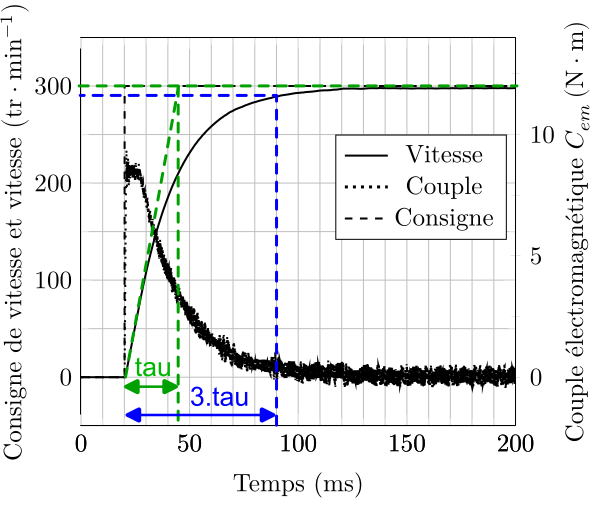
\includegraphics[width=0.6\textwidth]{img/cor17}
\end{center}

D'après le premier relevé de la figure 17, on a à régime permanent pour une consigne $N_c = 300$ tr$\cdot$min$^{-1}$ :
$$N_{m,\infty} = 300~\text{tr} \cdot \text{min}^{-1}$$

On a donc $K = \dfrac{N_{m,\infty}}{N_c} = \dfrac{\omega_{m,\infty}}{\omega_c} = 1$.

A l'aide de 3 méthodes, on peut identifier la constante de temps $\tau$ :
\begin{itemize}
\item à l'aide du temps de réponse à 5\% : $t_{5\%} \simeq 70$ ms $\Longrightarrow \tau = \dfrac{t_{5\%}}{3} \simeq 23,3$ ms ;
\item à l'aide de la tangente à l'origine : $\tau \simeq 24$ ms.
\end{itemize}}

\reponse{2}{}{Le codeur délivre 10000 points par tour soit :
$$K_{\text{cod}} = \frac{10000}{2\pi} \simeq 1592~\text{points} \cdot \text{rad}^{-1}$$

Pour assurer un bon asservissement, on doit avoir un écart $\varepsilon(p) = X_c(p) - X(p) = 0$ lorsque $X_c(p) = X(p)$ soit

$$\varepsilon(p) = A \cdot X_c(p) - K_{\text{cod}} \cdot \frac{X(p)}{\rho_x} = 0 \text{ pour } X_c(p) = X(p)$$

$$\Longrightarrow A = \frac{K_{\text{cod}}}{\rho_x}$$

\textbf{Application numérique :} $A \simeq 1{,}6 \times 10^5$ points$\cdot$m$^{-1}$}

\reponse{2}{}{La résolution du codeur vaut

$$\Delta\theta = \frac{1}{K_{\text{cod}}} \Longrightarrow \Delta\theta \simeq 6{,}3 \times 10^{-4}~\text{rad}$$

Ce codeur permettra donc de voir un déplacement :
$$\Delta x = \rho_x \cdot \Delta\theta$$

Soit $\Delta x \simeq 6{,}3~\mu$m $< 0{,}5$ mm. Cette résolution est donc bien compatible avec les exigences de précision demandée.}

\reponse{3}{}{D'après le schéma-bloc : $\text{FTBO}(p) = C(p) \cdot H(p) \cdot \dfrac{1}{p} \cdot K_{\text{cod}}$

Donc
$$\text{FTBO}(p) = \frac{K_p \cdot K_{\text{cod}}}{p \cdot (1 + \tau \cdot p)}$$}

\reponse{4}{\begin{center}
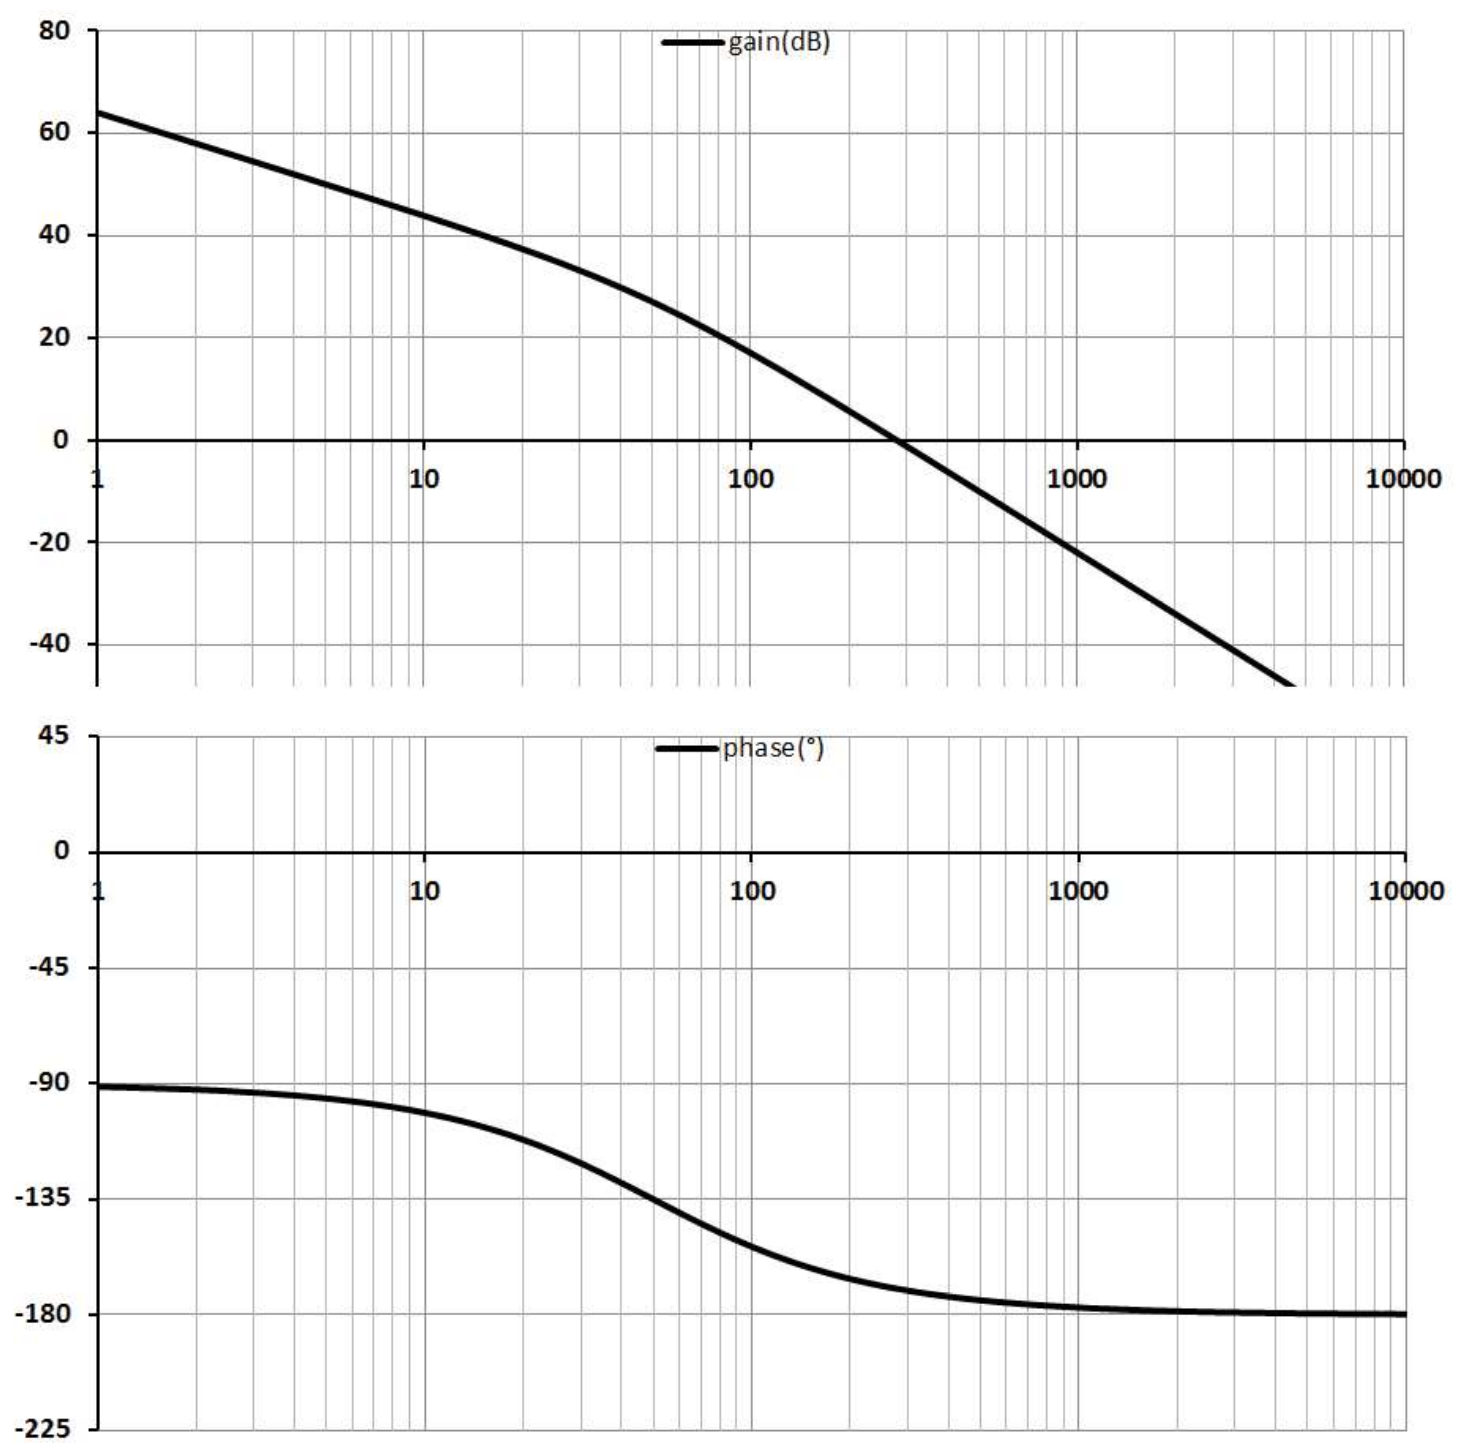
\includegraphics[width=0.6\linewidth]{img/dr29}
\end{center}}{
\begin{center}
 \def\svgwidth{0.8\linewidth}
 \input{img/cor29.pdf_tex}
\end{center}

On trouve $20\cdot log(K_p\cdot K_{cod})=64$, donc $K_p\cdot K_{cod}=10^{3,2}=1000* \sqrt[5]{10}\approx 1500$, on retrouve la valeur calculée précédemment.

On trouve $\dfrac{1}{\tau}=50$, soit $\tau=20ms$, c'est aussi la valeur trouvée précédemment.}

\reponse{3}{}{$$\text{FTBF}(p) = \frac{\frac{K_1}{p \cdot (1 + \tau \cdot p)}}{1 + \frac{K_1}{p \cdot (1 + \tau \cdot p)}} = \frac{K_1}{K_1 + p + \tau \cdot p^2}$$}

\reponse{3}{}{Par le théorème de la valeur finale :
\begin{align*}
\Delta x_v &= \lim_{p\to 0}p \cdot \mu(p)\\
&= \lim_{p\to 0}p \cdot (X_c(p) - X(p))
\end{align*}

Soit
\begin{align*}
\Delta x_v &= \lim_{p\to 0}\left(1 - \text{FTBF}(p)\right) \cdot \frac{V_x}{p}\\
&= \lim_{p\to 0}\frac{1 + \tau \cdot p}{K_1 + p + \tau \cdot p^2} \cdot V_x
\end{align*}

Donc
$$\Delta x_v = \frac{V_x}{K_1}$$}

\reponse{3}{}{On a d'après la question précédente $\Delta x_v \simeq 36$ mm $< 50$ mm.

Ainsi, le système est capable de suivre les lois d'évolution de position en translation, en prenant en compte les exigences du tableau de la figure \ref{fig02}.

Sur l'erreur statique, cette dernière sera nulle car la $\text{FTBO}(p)$ est de classe 1. Ces résultats respectent l'exigence de précision sur l'erreur pour une consigne en échelon.}

\end{document}